\documentclass[citation\_needed]{subfiles}
\begin{document}

Comme nous l'avons vu précédemment, les réseaux récurrents les plus couramment utilisés sont des variantes du réseau d'Elman. Il existe cependant d'autres types de réseaux récurrents pouvant être utilisés dans le TAL. Le premier est le réseau de \citet{jordan1986serial}. Ce réseau est une extension du réseau de Elman. Là où un réseau d'Elman a une connexion récurrente sur la couche cachée uniquement, la connexion récurrente d'un réseau de Jordan relie la couche de sortie à la couche cachée. L'utilisation de ce type de réseaux dans le cadre du TAL est plus justifiée car il permet de capturer des dépendances au niveaux des annotations.

Dans cette section, nous verrons principalement une variante de RNN récente : les LD-RNN \citep{dinarelli2016etude,dupont2017a}, une extension des réseaux d'Elman et Jordan. Les LD-RNN étendent le principe des réseaux d'Elman en reliant la couche de sortie directement à la couche d'\textit{embedding} du réseau. Ainsi, le réseau peut tirer au mieux parti des informations fournies par les étiquettes précédemment prédites, ces dernières passant par l'entièreté du réseau. Les différences entre un réseau d'Elman, de Jordan et un LD-RNN sont données dans la figure \ref{fig:3architecgtures}. Dans cette figure, $w$ représente les tokens, $y$ les étiquettes, et E, H, O et R sont les paramètres du modèle.

\begin{figure}[ht!]
    \begin{minipage}{0.325\linewidth}
    \centering
    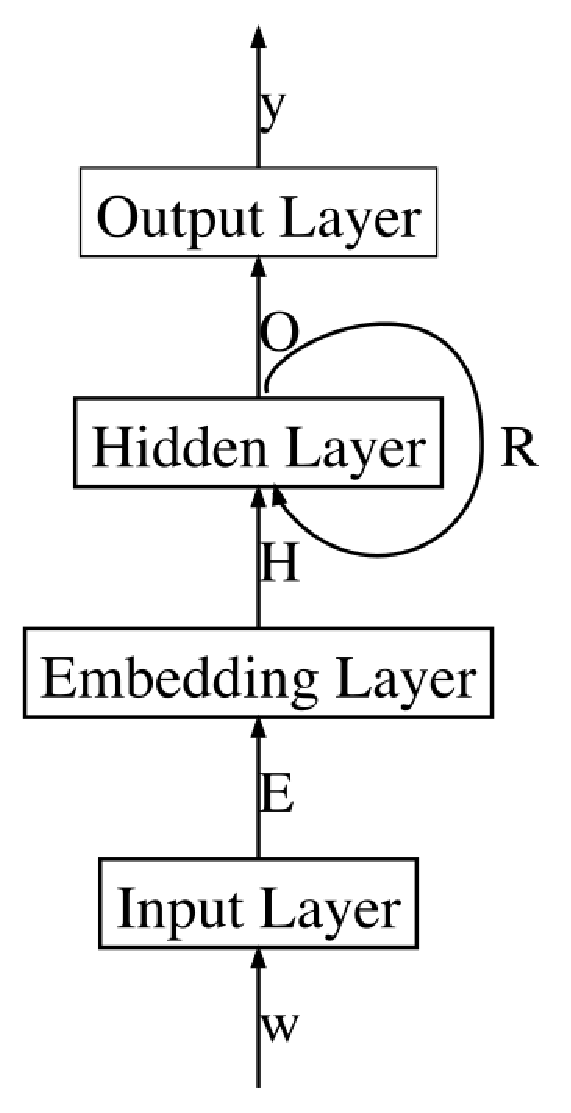
\includegraphics[scale=0.4]{images/NN/LD-RNN/ElmanRNN_inkscape}
    \end{minipage}
    \begin{minipage}{0.325\linewidth}
    \centering
    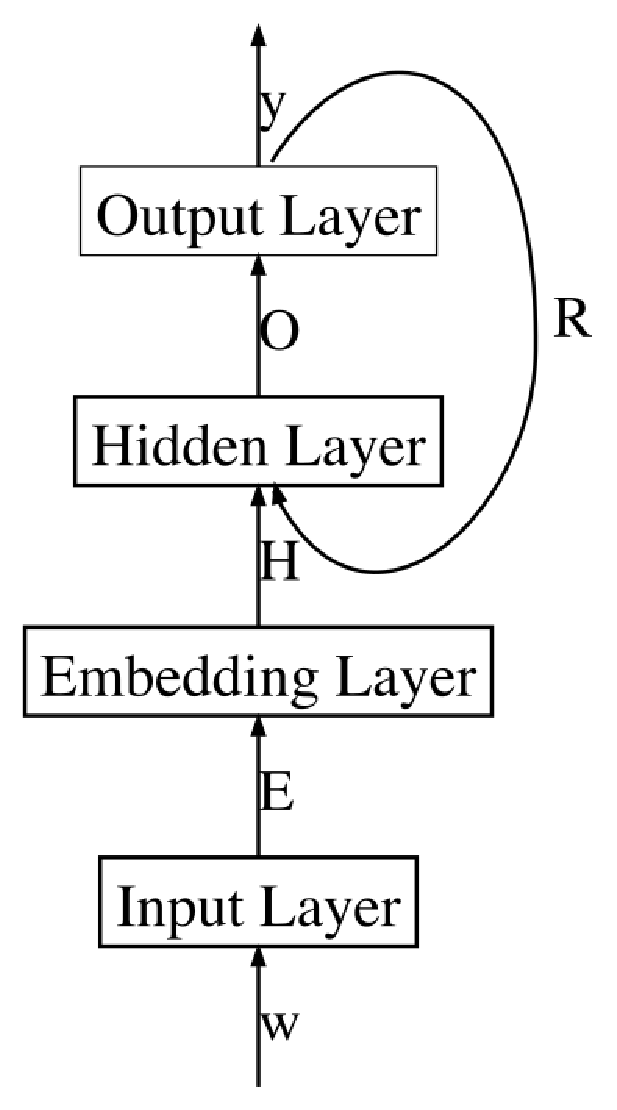
\includegraphics[scale=0.4]{images/NN/LD-RNN/JordanRNN_inkscape}
    \end{minipage}
    \begin{minipage}{0.325\linewidth}
    \centering
    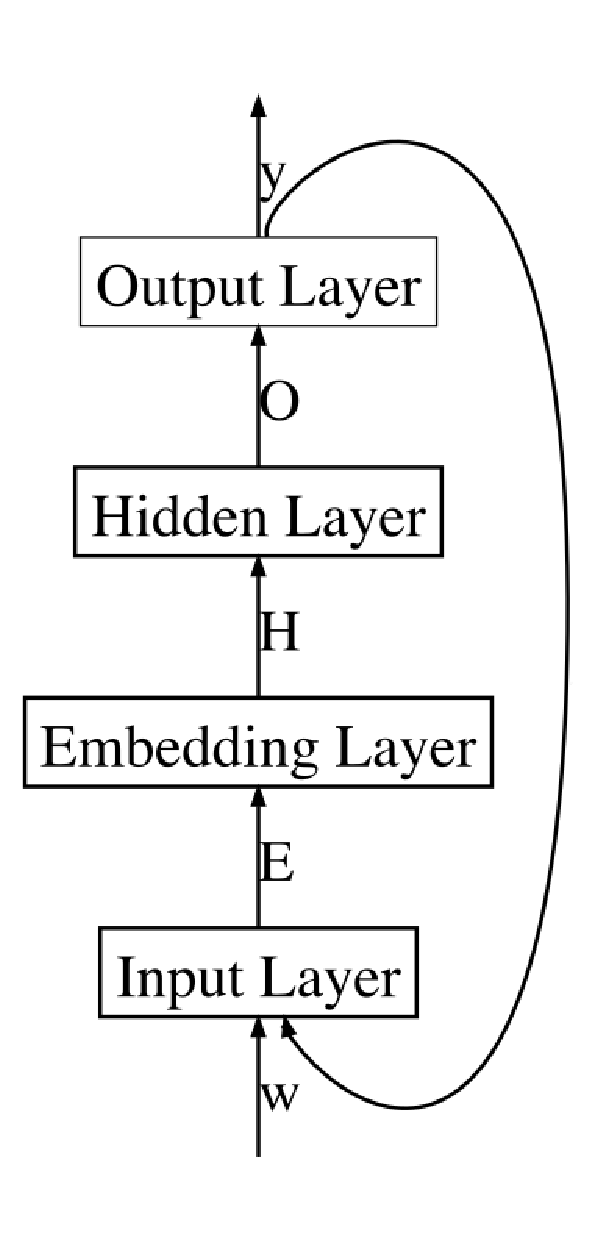
\includegraphics[scale=0.4]{images/NN/LD-RNN/OcramRNN_inkscape}
    \end{minipage}
    \caption{Schéma général des principaux RNN. À gauche, un réseau d'Elmann. Au centre, un réseau de Jordan. À droite, un LD-RNN. Image tirée de \citet{dupont2017a}.}
    \label{fig:3architecgtures}
\end{figure}

Comme nous l'avons vu précédemment, l'une des grandes forces des réseaux de neurones pour le TAL est leur utilisation de représentations. L'intérêt des LD-RNN est de renvoyer l'information de la couche de sortie à la couche \textit{embedding} (de représentation). Ainsi, il devient possible d'utiliser des représentations vectorielles pour les étiquettes, comme cela est également fait pour les tokens. Nous pouvons alors capturer le même type d'informations distributionnelles que pour les tokens. En effet, le calcul des étiquettes de sortie se fait à l'aide d'un \textit{softmax} décrit dans l'équation \ref{eq:softmax}. Nous pouvons transformer ce \textit{softmax} en représentation creuse dont la taille est le nombre d'étiquettes. Dans ce vecteur, toutes les valeurs sont égales à 0, sauf celle à l'indice de l'étiquette ayant la plus grande probabilité, qui aura alors une valeur de 1. Nous pouvons alors, de manière équivalente aux tokens, utiliser cette représentation creuse en tant qu'indice pour chercher dans une table de correspondances une représentation dense de l'étiquette. Il devient alors possible d'adapter la représentation des étiquettes afin de mieux s'adapter à la tâche cible par rétro-propagation. Utiliser des représentations denses d'étiquettes avait déjà été proposé par \citet{chen2014fast}, qui utilisaient des représentations préapprises dans le cadre de l'analyse sytnaxique en dépendances. Les LD-RNN vont plus loin dans le sens où ils prennent en compte un contexte étendu d'étiquettes qui, grâce à la rétro-propagation, permet d'apprendre les dépendances qui lient les étiquettes ainsi que d'extraire des features internes des étiquettes, en plus de celles des tokens.

Par soucis de simplicité, nous notons E$_{w}$ la matrice des représentations des tokens, et E$_{l}$ celle des représentations des étiquettes.

Le LD-RNN utilise, à l'instar d'un CNN présenté précédemment, des fenêtres de tokens pour avoir plus de contexte au moment de la prédiction. Ces fenêtres sont des contextes gauches et droits d'une taille fixée définie à l'avance $wd$. Nous notons $W_{t}$ le contexte au niveau des tokens du réseau qui est calculé comme suit :

\begin{equation}\label{eq:LD-RNN-word-window}
W_{t} = \left[ E_{w}(w_{t-wd})\ ...\ E_{w}(w_{t})\ ...\ E_{w}(w_{t+dw}) \right]
\end{equation}

Où les crochets $[\ ]$ représentent l'opération de concaténation et $w_{t}$ l'indice dans le vocabulaire du token à la position t de la séquence.

$L_{t}$ est quant à lui le contexte au niveau des étiquettes du réseau et sa définition la plus simple, qui ne tient compte que de l'étiquette précédente, est donc :

\begin{equation}\label{eq:LD-RNN-minimal}
L_{t} = E_{l}(y_{t-1})
\end{equation}

Où y$_{t}$ est l'indice de l'étiquette la plus probable à l'instant t. Ainsi, le réseau prend en compte, à chaque instant t, l'étiquette prédite à l'instant précédent. Cette définiton se généralise alors naturellement pour prendre en compte un nombre fixé et donné à l'avance $c$ d'étiquettes de contexte, de la façon suivante :

\begin{equation}\label{eq:LD-RNN-label-window}
L_{t} = \left[ E_{l}(y_{t-c})\ ...\ E_{l}(y_{t-1}) \right]
\end{equation}

Cette taille de contexte arbitraire permet d'obtenir des modèles plus informatifs que les CRF, qui ne prennent qu'une seule étiquette de contexte (en plus de l'étiquette courante). Il n'est cependant pas garanti que cette accumulation des étiquettes de contexte soit plus puissante que celle des CRF, le calcul de l'étiquette courante se faisant de façon locale pour l'étiquette courante dans le LD-RNN, alors que pour le CRF ce calcul est global sur l'ensemble de la séquence.

Les contextes $W_{t}$ et $L_{t}$ sont calculés de manière séparée et passent chacun dans une couche cachée leur étant propre, $H_{w}$ et $H_{l}$ respectivement pour les tokens et les étiquettes, afin de donner une représentation interne qui sera utilisée dans le réseau. Ces deux représentations sont alors concaténées en une nouvelle qui est passée dans une seconde couche cachée globale, $H$, son calcul étant alors :

\begin{equation}\label{eq:LD-RNN-hidden}
H_{t} = \phi(\left[ (H_{w} \times W_{t})\ (H_{l} \times L_{t}) \right])
\end{equation}

Où $\phi$ est une fonction d'activation. Un schéma du calcul de $H_{t}$ est donné dans la figure \ref{fig:ht-computation}.

\begin{figure}[ht!]
    \centering
    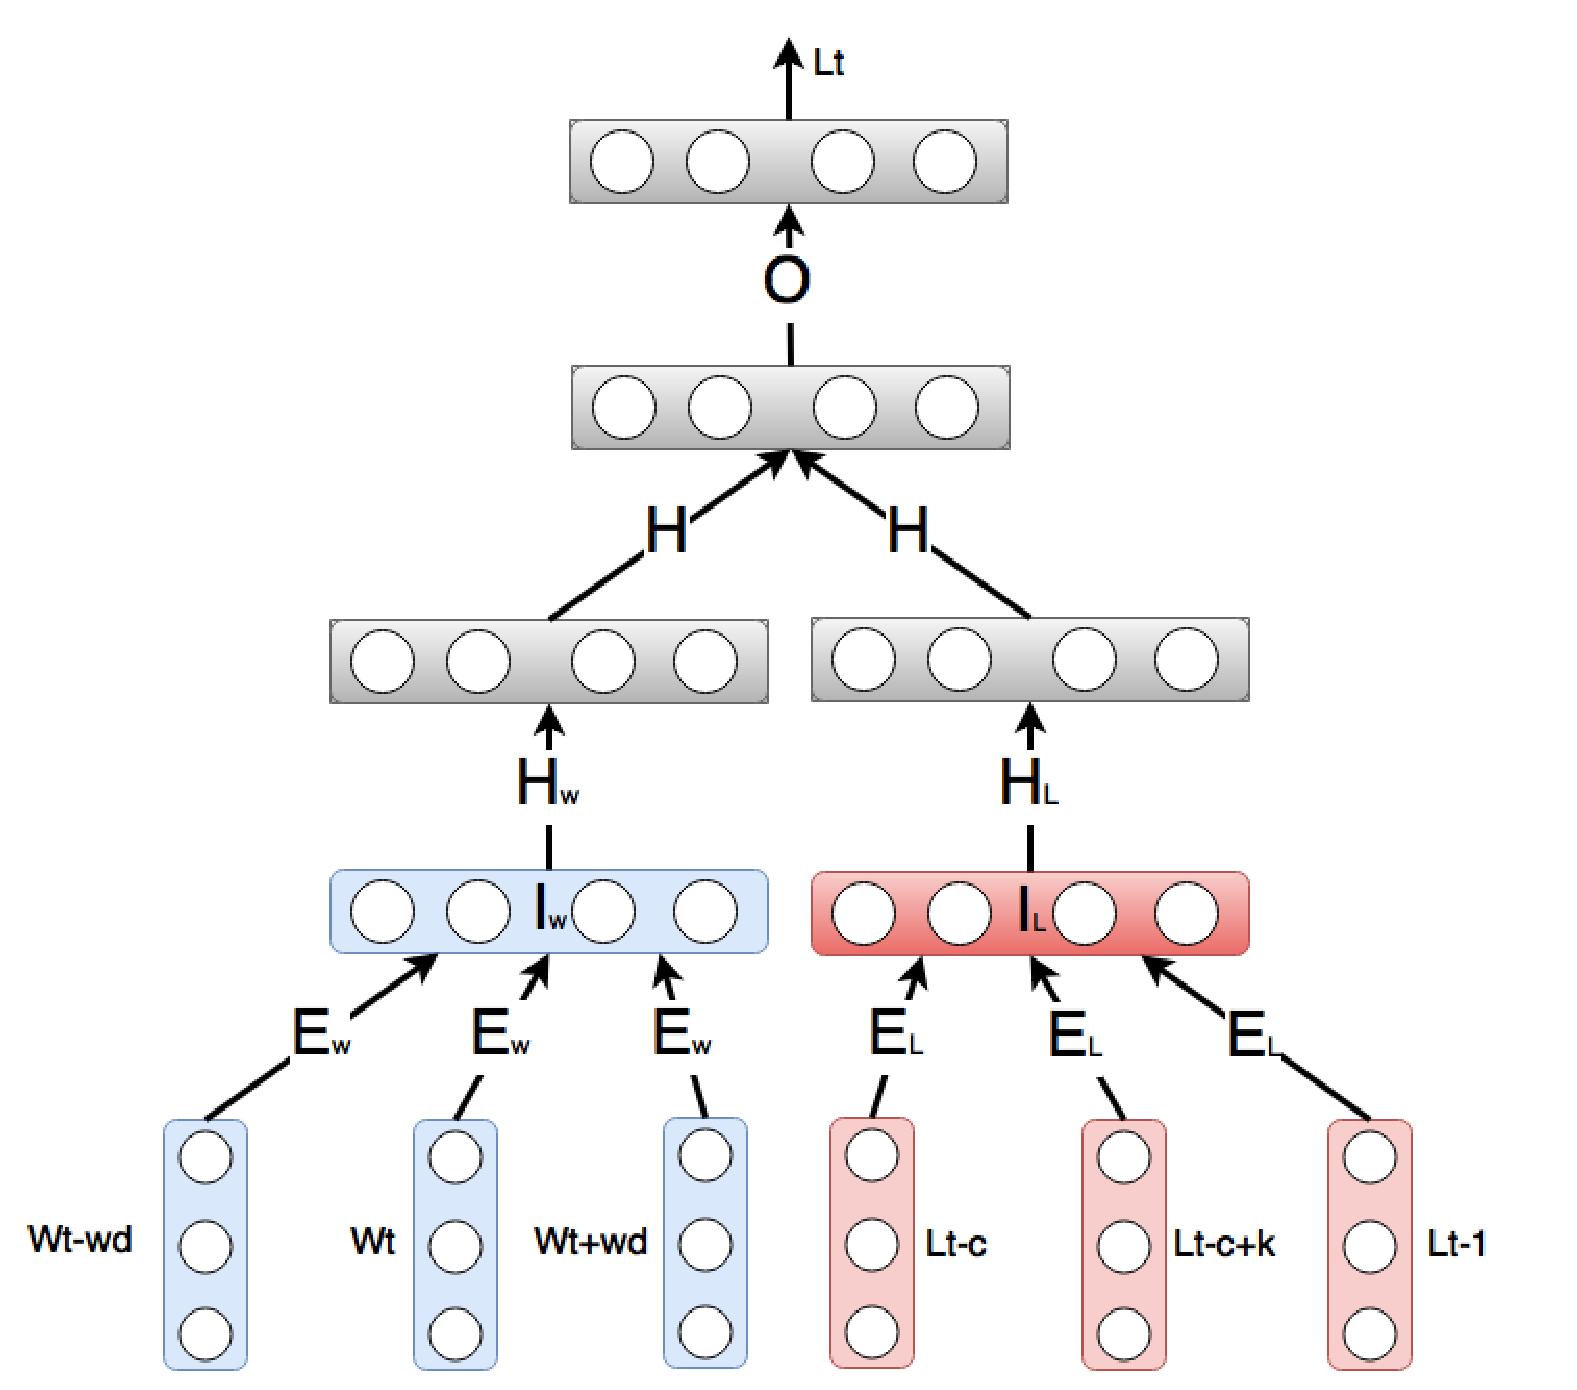
\includegraphics[scale=0.3]{images/NN/LD-RNN/DeepLDRNN_2}
    \caption{une représentation graphique du calcul de la couche cachée d'un LD-RNN. Schéma tiré de \citet{dupont2017a}.}
    \label{fig:ht-computation}
\end{figure}

Ces réseaux permettent de corriger certains problèmes présents dans des réseaux de neurones comme les LSTM, tout en restant computationellement plus simples. Ces réseaux étant arrivés tardivement dans la thèse, nous n'avons pas pu les tester sur les corpus présentés dans la section \ref{chap:NER-corpus}. Cependant, ils sont parvenus à obtenir des performances état-de-l'art sur les corpus ATIS et MEDIA dans le domaine de la compréhension de la parole \ref{dupont2017a,dinarelli2017modelisation}, battant les CRFs et les autres réseaux récurrents comme LSTM et GRU.

Chaque type de réseau de neurone offre des avantages et des inconvénients qui lui sont propres. Certains réseaux s'inspirent également d'autres technologies et intègrent des couches répliquant leur fonctionnement. Dans la prochaine section, nous détaillerons ces systèmes de réseaux de neurones combinés.
%La seconde étant de combiner différents modèles de NN (principalement) pour que les différents réseaux profitent des avantages des autres.

\end{document}